\documentclass[a4paper,10pt]{ctexart}
%引用设置使用Bibtex
\usepackage{gbt7714}
\bibliographystyle{gbt7714-numerical}
%页面设置
\usepackage{geometry}
%字体设置
\usepackage{fontspec}
%\setmainfont{Times New Roman}
%定理环境
\usepackage{amsmath}
\numberwithin{equation}{section}
\usepackage{amsthm}
\newtheorem*{definition}{Definition}
\newtheorem{theorem}{Theorem}
\newtheorem{lemma}{Lemma}
\newtheorem*{corollary}{Corollary}
\newtheorem*{proposition}{Proposition}
\newtheorem*{example}{Example}
%数学环境字体
\usepackage{bm}
\usepackage[all]{xy}
%加载 TikZ 用于绘制交换图
\usepackage{tikz-cd}
\usepackage{tikz}
\usepackage{pgfplots}
\newcommand{\tikzdef}{\pgfmathsetmacro} % 在tikzpicture内的foreach循环中定义实数临时变量
%颜色
\usepackage{color,xcolor}

\definecolor{miku}{RGB}{57,197,187}
\definecolor{sakura}{RGB}{255,192,203}
\definecolor{rose}{RGB}{255,228,225}
\definecolor{brown}{RGB}{210,105,30}
\definecolor{lbrown}{RGB}{239,235,224}
\definecolor{bule}{RGB}{0,47,167}
\definecolor{lyellow}{RGB}{250,250,210}
\definecolor{lpurple}{RGB}{255,240,245}
\definecolor{lbule}{RGB}{135,206,250}
\definecolor{gbule}{RGB}{64,224,208}
\definecolor{green}{RGB}{138,200,207}
\definecolor{lgreen}{RGB}{225,255,255}
\definecolor{lorange}{RGB}{248,172,140}
\definecolor{salmon}{RGB}{250,128,114}
\definecolor{burgundy}{rgb}{0.5, 0.0, 0.13}
%链接设置
\usepackage[colorlinks=true,pdfstartview=FitH,linkcolor=blue,anchorcolor=violet, citecolor=magenta]{hyperref} 
%封面
\usepackage{pdfpages}
\usepackage{mathrsfs}
\usepackage{amssymb}
\usepackage{graphicx}
\usepackage{lipsum}
%彩色框
\usepackage{framed}
\usepackage{tcolorbox}
\tcbuselibrary{breakable}
\tcbuselibrary{theorems}
\tcbuselibrary{skins}
\usepackage{colortbl}
\usepackage{float}
\usepackage[export]{adjustbox}
\newtcolorbox[auto counter,number within=section]{notebox}[2][]{%
colback=miku!2!white,
colframe=miku,
coltitle=white,
fonttitle=\bfseries,
rightrule=2pt,
leftrule=2pt,
bottomrule=2pt,
colbacktitle=miku,
theorem style=standard,
breakable,
arc=2pt,
drop fuzzy shadow=black!20!white,
title=Note~\thetcbcounter: #2,#1}
\newtcolorbox[auto counter,number within=section]{markbox}[2][]{%
colback=miku!2!white,
colframe=miku,
coltitle=white,
fonttitle=\bfseries,
rightrule=0pt,
leftrule=0pt,
bottomrule=2pt,
colbacktitle=miku,
theorem style=standard,
breakable,
arc=0pt,
drop fuzzy shadow=black!20!white,
title=Remark~\thetcbcounter: #2,#1}
\newtcolorbox[no counter]{theorems}[2][]{%
width=12cm,
center,
sidebyside,
sidebyside adapt=left,
sidebyside gap=6mm,
sidebyside align=center seam,
colback=burgundy!2!white,
colframe=burgundy,
coltitle=white,
fonttitle=\bfseries,
rightrule=1pt,
leftrule=1pt,
bottomrule=2pt,
colbacktitle=burgundy,
theorem style=standard,
enhanced,
drop fuzzy shadow southeast=black!30!white,
breakable,
arc=0pt,
title=Theorem. #2,#1}
\newtcolorbox[no counter]{definitions}[2][]{%
width=12cm,
center,
colback=lyellow!2!white,
colframe=yellow!3!lyellow,
coltitle=bule,
fonttitle=\bfseries,
rightrule=0pt,
leftrule=1pt,
bottomrule=2pt,
colbacktitle=lyellow,
theorem style=standard,
breakable,
arc=5pt,
enhanced,
drop fuzzy shadow southeast=black!20!white,
title=Definition. #2,#1}
\newtcolorbox[auto counter,number within=section]{corollarys}[2][]{%
colback=lyellow!2!white,
colframe=lyellow,
coltitle=bule,
fonttitle=\bfseries,
rightrule=0pt,
leftrule=1pt,
bottomrule=2pt,
colbacktitle=lyellow,
theorem style=standard,
breakable,
arc=0pt,
enhanced,
drop fuzzy shadow southeast=black!20!white,
title=Corollary~\thetcbcounter: #2,#1}
\newtcolorbox[auto counter,number within=section]{lemmas}[2][]{%
width=12cm,
center,
colback=lyellow!2!white,
colframe=lorange!30!sakura,
coltitle=bule,
fonttitle=\bfseries,
rightrule=0pt,
leftrule=1pt,
bottomrule=2pt,
colbacktitle=lorange!30!sakura,
theorem style=standard,
breakable,
arc=5pt,
enhanced,
drop fuzzy shadow southeast=black!20!white,
title=Lemma. #2,#1}
\newtcolorbox[auto counter,number within=section]{propositions}[2][]{%
width=12cm,
center,
colback=salmon!5,
colframe=salmon!90!black,
coltitle=white,
fonttitle=\bfseries,
rightrule=1pt,
leftrule=1pt,
bottomrule=2pt,
colbacktitle=salmon!90!black,
theorem style=standard,
breakable,
arc=5pt,
enhanced,
drop fuzzy shadow southeast=black!20!white,
title=Proposition. #2,#1}
\newtcolorbox[no counter]{egbox}[2][]{%
width=12cm,
center,
colback=black!5!white,
colframe=black!20!white,
coltitle=black,
fonttitle=\bfseries,
rightrule=1pt,
leftrule=1pt,
bottomrule=2pt,
colbacktitle=black!20!white,
theorem style=standard,
breakable,
arc=0pt,
enhanced,
drop fuzzy shadow southeast=black!20!white,
title=Example. #2,#1}

%\begin{figure}[H]
%\centering
%\includegraphics[center]{pic.png}
%\end{figure}
\geometry{left=3cm,right=3cm,top=2cm,bottom=2cm}
\tcbuselibrary{most}

\usepackage[linesnumbered,ruled,vlined]{algorithm2e}
\usepackage{algorithmic}

\SetKwProg{Fn}{function}{\string:}{}
\newcommand{\forcond}{$i=0$ \KwTo $n$}
\SetKwFunction{FRecurs}{FnRecursive}
\SetKwInput{KwCost}{Cost}

\usepackage{holtpolt}

%自定义设置
\renewcommand{\proofname}{Proof.}
\renewcommand{\contentsname}{ Content }
\newcommand{\image}[2]{
    \centering
    \includegraphics[width={#1}\textwidth]{#2}
}



\newcommand\keywords[1]{\vskip2ex\par\noindent\normalfont{\textbf{关键词}: #1}}
\newcommand{\ekeywords}[1]{\vskip2ex\par\noindent\normalfont{\bfseries Key Words: }#1}
\newcommand{\miku}{\textcolor{miku}}
\newcommand{\sakura}{\textcolor{sakura}}
\newcommand{\brown}{\textcolor{brow}}
\newcommand{\red}{\textcolor{red}}
\newcommand{\blue}{\textcolor{blue}}
\newcommand{\A}{\mathcal{A}}
\newcommand{\C}{\mathbb{C}}
\newcommand{\al}{\alpha}
\newcommand{\sa}{$\sigma$-algebra}
\newcommand{\Bsa}{Borel $\sigma$-algebra}
\newcommand{\F}{\mathcal{F}}
\newcommand{\N}{\mathcal{N}}
\newcommand{\M}{\mathcal{M}}
\newcommand{\m}{ $\mathcal{M}$ }
\newcommand{\B}{\mathcal{B}}
\newcommand{\myP}{\mathcal{P}}
\renewcommand{\bf}[1]{\textbf{#1}}

\newcommand{\myRom}[1]{\uppercase\expandafter{\romannumeral#1}}
\newcommand{\pl}{$ L^p(X) $}
\newcommand{\twol}{$ L^2(X) $}

\usepackage{booktabs}
\usepackage{arydshln}

\begin{document}
\hfill\vbox{\hbox{Numerical Analysis}\hbox{陈曦,UESTC}\hbox{Summer, 2024}}

\begin{center}\Large
    \textbf{数值线性代数}\\{\normalsize\bf {最小二乘问题和特征值问题}}
\end{center}
\vskip 30pt
\small {参考书目:
\begin{itemize}
    \item Accuracy and Stability of Numerical Algorithms(Higham,2002)
    \item Fundamentals of Matrix Computations(Watkins,2010)
    \item 数值线性代数(徐树方,2013)
\end{itemize}}

本文首先介绍矩阵的QR分解,然后讨论两类重要并且相互联系的问题:最小二乘问题和特征值问题。最小二乘本质上是在寻找子空间上的最佳投影,而QR分解则为此提供了一种有力的工具,以QR分解为基础的QR算法也为寻找特征值提供了一种高效的方法。在第一部分,我们将主要介绍正交变换法来求解最小二乘问题,主要的工具包括Householder变换、Givens变换等。而第二部分则从古典的幂法和反幂法开始,之后介绍QR算法。

\section{QR分解}
QR分解是一种重要的矩阵分解工具,在数值计算中有着广泛的应用,可以用来求解线性方程组,寻找最小二乘解,并且是用来求解特征值问题的QR迭代算法的基础。

如果$ A\in \mathbb{R}^{m\times n} $,其中$ m\geqslant n $,则如下分解称为$ A $的QR分解:
\begin{equation}
    A = QR = 
    \begin{bmatrix}
        Q_1 & Q_2
    \end{bmatrix}
    \begin{bmatrix}
        R_1\\
        0
    \end{bmatrix} = Q_1 R_1,
\end{equation}
其中$ Q\in \mathbb{R}^{m\times m} $是正交矩阵,$ R_1\in \mathbb{R}^{n\times n} $是一个上三角矩阵。其中$ Q_1R_1 $是$ QR $的等价的紧凑形式,两者都称做是$ A $的QR分解。值得注意的是,$ Q_1 $的各列是$ R(A) $的一组标准正交基,而$ Q $的各列则是$ \mathbb{R}^m $的一组标准正交基。

使用Cholesky分解可以证明QR分解的存在性。如果$ A $是满秩矩阵,则$ A^TA\in \mathcal{S}_{++} $,于是$ A^TA $有Cholesky分解$ A^TA = R^T R$,于是可以验证$ Q = AR^{-1} $的各列互相标准正交,于是$ A = AR^{-1}\cdot R $就是$ A $的QR分解。当$ A $满秩且$ R $的对角元都是正数时(令$ A = QD\cdot DR $,$ D = \operatorname{diag}(\pm 1) $),如上构造的QR分解是唯一的。

通常而言要得到矩阵的QR分解有三种方法:
\begin{itemize}
    \item Gram-Schmit正交化方法:这是最古老的QR分解算法,根据实现的区别分为经典Gram-Schmidt方法(CGS)和修正Gram-Schmidt方法(MGS);
    \item Givens旋转:这种方法可以在矩阵内部引入零元素,从而实现QR分解。这一方法特别适合于具有稀疏结构的矩阵;
    \item Householder变换:这是对于一般矩阵而言最有用的QR分解方法,本质上是一种投影方法。
\end{itemize}
我们下面依次介绍这三种方法。
\subsection{Householder变换}
Householder矩阵形如
\begin{equation}
    P = I - \frac{2vv^T}{v^T v},
\end{equation}
是一个对合矩阵($ P^2 = I $),同时满足对称性$ P^T = P $和正交性$ P^T P = I $。任意$ x\in \mathbb{R}^n $
\[
    Px = x - \frac{2v^T x}{v^T v}v,
\]
不难看出$ Px $是$ x $关于超平面$ {\rm span}(v)^\perp $的镜像,因为
\[
    x - Px = \frac{2v^T x}{v^T v}v \in {\rm span}(v),
\]
$ (x + Px) / 2 = x - (v^T x)/(v^Tv)v $是$ x $在超平面$ {\rm span}(v)^\perp $上的投影,如图\ref{fig:Householder}所示。该投影过程可以视作先将$ x $投影到$ v $方向上,然后从$ x $中减去两倍的这一投影以实现关于$ {\rm span}(v)^\perp $的反射。
\begin{figure}[htpb]
    \centering
    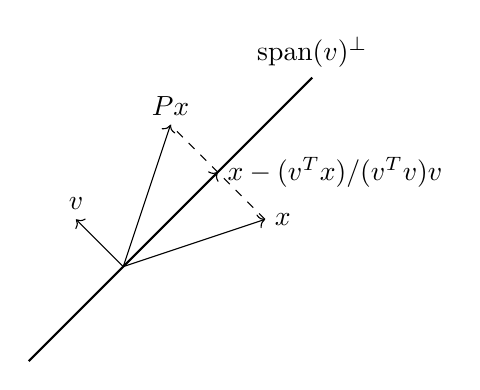
\begin{tikzpicture}[scale=0.6]
        \draw[->] (0,0) -- (-1,1) node[above] {$v$};
        \draw[->] (0,0) -- (3,1) node[right] {$x$};
        \draw[->] (0,0) -- (1,3) node[above] {$Px$};
        \draw[dashed] (3,1) -- (1,3);
        \draw[->] (0,0) -- (2,2) node[right] {$x - (v^T x)/(v^Tv)v $};
        \draw[thick] (-2,-2) -- (4,4) node[above] {${\rm span}(v)^\perp$};
    \end{tikzpicture}
    \caption{Householder矩阵作用在某一向量$ x $上}
    \label{fig:Householder}
\end{figure}

给定两个不同的向量$ x $和$ y $,如果它们的范数相同$ \| x \|_2 = \| y \|_2 $(因为$ P $是保矩的,所以范数相同是必要条件),我们可以通过Householder变换将$ x $变换为$ y $:令$ v = x - y $,则相应的Householder矩阵为
\[
    P = I - \frac{2(x - y)(x - y)^T}{(x - y)^T(x - y)} = I - \frac{2(x - y)(x - y)^T}{\| x - y \|_2^2},
\]
直接验证可知$ Px = y $。在实际应用中,通常令$ y $是一些具有特殊结构(有一些零)的向量,最常见的是令$ y = \sigma e_1 $,其中$ |\sigma| = \| x \|_2 $以保证相应的Householder矩阵是存在,此时的$ v = x - \sigma e_1 $,为了避免在计算两个相近的数相减时会出现的灾难性抵消现象(有效数字个数下降),通常令
\[
    \sigma = - {\rm sign}(x_1) \| x \|_2,
\]
于是$ v = x + {\rm sign}(x_1) \| x \|_2 e_1 $从而避免出现了减法;另一种做法如算法\ref{alg:Householder}所示,令$ \sigma = {\rm sign}(x_1) \| x \|_2 $,但是通过计算如下等价的公式来得到$ v $以避免减法的出现:
\begin{equation}\label{eq:Householder}
    v_1 = x_1 - \sigma = \frac{x_1^2 - \| x \|_2^2}{x_1+\sigma} = \frac{-(x_2^2 + \cdots + x_m^2)}{x_1+\sigma}.
\end{equation}

\begin{algorithm}[htbp]
    \caption{Householder Transform}\label{alg:Householder}
    \KwData{nonzero vector $ x\in \mathbb{R}^{n} $.}
    \KwResult{$ v $ and $ \beta = 2 / (v^Tv) $ s.t. $ Px = \sigma e_1 $ where $ P = I- \beta vv^T $, $ \sigma ={\rm sign}(x_1) \| x \|_2 $.}
    Preconditioning: $ \eta = \| x \|_\infty, \ x = x / \eta $\;
    $ (v_2,\cdots ,v_n) = (x_2,\cdots,x_n) $\;
    $ \alpha = (x_2,\cdots ,x_n)^T (x_2,\cdots ,x_n) $\;
    \eIf{$ \alpha = 0 $}{
        $ \beta = 0 $\tcc*[c]{$ x={\rm sign}(x_1)\| x \| e_1,\quad P=I $}
    }{
        $ \sigma = \sqrt{x_1^2 + \alpha} $\;
        \If{$ x_1\leqslant 0 $}{
            $ \sigma = -\sigma $\;
        }
        $ v_1 = -\alpha / (x_1+\sigma) $ \tcc*[c]{use \eqref{eq:Householder}}
        $ v = v / v_1 $ \tcc*[c]{normalize $ v $}
        $ \beta = 2 / (v^Tv) $\;
    }
    \Return $ v,\ \beta $\;
\end{algorithm}

算法\ref{alg:Householder}中最后一步令$ v $的首个元素标准化为$ 1 $,这一操作使得此时无需再储存$ v_1=1 $,所以可以直接将$ v_2,\cdots ,v_n $储存在$ Px $的后$ n-1 $个元素中(根据$ P $的构造,这些元素已知为0),这样可以节省一些内存。

下面我们使用Householder变换来实现QR分解。一般地,通过依次在$ A\in \mathbb{R}^{m\times n} $上左作用上$ n $个Householder矩阵,我们可以将$ A $变换为一个上三角矩阵$ R $。令$ A_1 = A $,如果在第$ k $阶段的开始得到的
\[
    A_k = 
    \begin{bmatrix}
        R_{k-1} & z_k & B_k\\
        0 & x_k & C_k
    \end{bmatrix},\quad R_{k-1}\in \mathbb{R}^{(k-1)\times (k-1)},\quad x_k\in \mathbb{R}^{m-k+1},
\]
其中$ R_{k-1} $是上三角矩阵,现在我们需要选取一个Householder矩阵$ \tilde{P}_k $,使得$ \tilde{P}_k x_k = \sigma e_1^{(k)} $,并且令
\[
    P_k = 
    \begin{bmatrix} 
         I_{k-1} & \\
         & \tilde{P}_k
    \end{bmatrix},
\]
于是得到的$ P_k A_k = A_{k+1} $的左上角有一个$ k $阶的上三角矩阵。继续这一过程就得到了$ A $的QR分解,其中
\begin{equation}
    R = P_n P_{n-1}\cdots P_1 A = Q^T A.
\end{equation}
这一过程总共需要进行$ 2n^2(m-n / 3) $次浮点运算。

在实际计算中,各个$ P_i $不会被显式地构造,出于存储和计算的效率考虑,我们只储存相应的$ v_i $来进行计算。例如在计算$ A_{k+1} = P_k A_k $时,由于
\[
    \begin{bmatrix} 
        I_{k-1} & \\
        & \tilde{P}_k
    \end{bmatrix}
    \begin{bmatrix}
         R_{k-1} & z_k & B_k\\
         0 & x_k & C_k
    \end{bmatrix} =
    \begin{bmatrix}
        R_{k-1} & z_k & B_k\\
        0 & e_1^{(k)} & \tilde{P}_k C_k
    \end{bmatrix},
\]
所以我们只需要更新$ C_k $到
\[
    \tilde{P}_k C_k = (I - \beta v_k v_k^T)C_k = C_k - \beta v_k(v^T_k C_k), \beta = \frac{2}{v^T_kv_k},
\]
其中我们通过利用矩阵乘法的结合律使用矩阵-向量积代替了矩阵-矩阵积,这一操作可以显著地减少计算量。

如果希望获得使得$ A=QR $的$ Q $矩阵,则需要计算$ Q = P_1 P_2\cdots P_n $,由于$ P_i $中有效的$ \tilde{P}_i $的阶数随着$ i $增长而减小,从右到左相乘相比于从左到右相乘更加高效。不过对于大多数应用而言,我们并不需要显式地计算$ Q $,只需要记录下各$ v_i $和最终得到的$ R $即可。

\begin{algorithm}[htbp]
    \caption{QR factorization by Householder Transform}\label{alg:HouseholderQR}
    \KwData{$ A\in \mathbb{R}^{m\times n} $ of rank $ n \ (m\geqslant n) $. }
    \KwResult{QR factorization of $ A $.}
    \For{$ j=1:n $}{
        \If{$ j<m $}{
            $ [v_j,\beta_j] = \text{Householder}(A(j:m,j)) $ \tcc*[c]{use algorithm \ref{alg:Householder}}
            $ A(j:m,j:n) = A(j:m,j:n) - \beta v_j(v_j^TA(j:m,j:n)) $\;
            $ A(j+1:m,j) = v_j(2:m-j+1) $\;
        }
    }
    \Return {$ R = {\rm triu}(A) $ (upper triangluar part of A), $ \beta\in \mathbb{R}^{n} $, $ v_j\in \mathbb{R}^{m-j+1} $ is stored in $ j $th column of $ {\rm stril}(A) $ (strict lower triangluar part of A) with first elemet being $ 1 $}\;
    \KwCost {$ 2n^2(m - n / 3) $ flops.}
\end{algorithm}

由于在第$ i $个阶段将$ A $的第$ i $列下方变为零之后就不再需要原本$ A $这一列了,因此没必要继续保留$ a_i $只需要储存这一过程中用到的Householder变换($ v_i $和$ \beta $)和得到的$ r_i $。出于这一原因,在算法\ref{alg:HouseholderQR}中,我们将每次用于生成Householder矩阵的$ v_j $(第一个分量为1无需储存,只需储存后$ m-j $个分量)储存在$ A $的严格下三角部分($ A(j+1:m,j) $)中,将$ r_i $(后$ m-j $个分量均为零无需储存)储存在$ A $的上三角部分($ A(1:j,j) $)中,$ \beta $额外储存在一个向量中,如下式所示($ A\in \mathbb{R}^{4\times 3} $的例子),其中$ v_j = (1, v_{j+1,j},\cdots ,v_{mj})^T $。
\[
    A\longrightarrow
    \begin{bmatrix} 
        r_{11} & r_{12} & r_{13}\\
        v_{21} & r_{22} & r_{23}\\  
        v_{31} & v_{32} & r_{33}\\
        v_{41} & v_{42} & v_{43}\\
    \end{bmatrix},
    \quad \beta =
    \begin{bmatrix}
        \beta_1\\
        \beta_2\\
        \beta_3
    \end{bmatrix}.
\]

\subsubsection{基于Householder变换的QR分解稳定性}
总的来说,Householder变换在数值上是相当稳定的:无论是对某个向量进行Householder变换,还是计算Householder变换矩阵与其他矩阵的乘积,在范数意义下都是稳定的,并且最重要的基于Householder变换的QR分解在范数意义下也是后向稳定的。

为了方便起见,定义
\[
    \tilde{\gamma}_k = \frac{cku}{1-cku},
\]
其中$ c $是某个较小的常数。

\subsection{Givens旋转}
Givens旋转是另一种进行QR分解的方法,它通过不断地向矩阵$ A $中引入零元素来得到上三角结构以实现QR分解,为此需要构造Givens矩阵$ G(i,j,\theta)\in \mathbb{R}^{n\times n} $($ i\ne j $),该矩阵形如
\[
    G(i,j,\theta) = 
    \begin{bmatrix}
        I_{\min\{i,j\}-1} & & & &\\
        & c & & s &\\
        & & I_{|i-j|-1} & &\\
        & -s & & c & \\
        & & & & I_{n-\max\{i,j\}}
    \end{bmatrix},
\]
它的第$ i,j $行和$ i,j $列相交构成的$ 2\times 2 $子矩阵如下所示:
\[
    G([i,j], [i,j]) = 
    \begin{bmatrix}
        c & s\\
        -s & c
    \end{bmatrix},
\]
其中$ c=\cos \theta, s= \sin \theta $,其他的元素与单位矩阵$ I_n $相同。从几何上看,$ y = G(i,j,\theta)x $是将$ x $在平面$ {\rm span}(e_i,e_j) $内顺时针旋转$ \theta $后得到的向量,即
\[
    \begin{bmatrix} 
        y_i \\ y_j
    \end{bmatrix} = 
    \begin{bmatrix}
        c & s\\
        -s & c
    \end{bmatrix}
    \begin{bmatrix}
        x_i \\ x_j
    \end{bmatrix},\quad y_{k} = x_k\ (k\ne i,j).
\]
为了令旋转之后的$ y_j =0 $,需要令
\begin{equation}
    s = \frac{x_j}{\sqrt{x_i^2 + x_j^2}},\quad c = \frac{x_i}{\sqrt{x_i^2 + x_j^2}},
\end{equation}
此时$ y_i = cx_i+sx_j $。上式说明要构造$ G(i,j,\theta) $只需要$ x_i,x_j $,无需计算出角度$ \theta $,因此也简记$ G(i,j,\theta) = G_{ij} $。使用这一方法可以依次的令矩阵的下三角区域的元素变为零从而最终得到一个上三角矩阵$ R $。


\begin{algorithm}[htbp]
    \caption{Givens Rotation}\label{alg:Givens}
    \KwData{$ a,b\in \mathbb{R} $.}
    \KwResult{$ c,s $ s.t. $ \begin{bmatrix} 
        c & s\\
        -s & c
    \end{bmatrix} 
    \begin{bmatrix} 
        a \\ b 
    \end{bmatrix} = 
    \begin{bmatrix} 
        r \\ 0
    \end{bmatrix} $.}
    \eIf{$ b=0 $}{
        $ c=1,\ s=0 $\;
    }{
        \eIf{$ |b|>|a| $}{
            $ \tau = a/b,\ s = 1/\sqrt{1+\tau^2},\ c = s\tau $ \tcc*[c]{avoid near 0 division}
        }{
            $ \tau = b/a,\ c = 1/\sqrt{1+\tau^2},\ s = c\tau $ \tcc*[c]{avoid near 0 division}
        }
    }
    \Return $ c,s $\;
\end{algorithm}

注意到如果$ i_1, i_2,j_1,j_2 $互不相同,则$ G_{i_1,j_1}G_{i_2,j_2} = G_{i_2,j_2}G_{i_1,j_1} $可交换,此时称$ G_{i_1,j_1} $和$ G_{i_2,j_2} $是不相交的。当$ G_{i_1,j_1} $和$ G_{i_2,j_2} $不相交时,$ G_{i_2,j_2}G_{i_1,j_1}A $可以并行地计算:
\[
    A([i_1,j_1],[i_1,j_1]) \leftarrow G_{i_1,j_1}A([i_1,j_1],[i_1,j_1]),\quad A([i_2,j_2],[i_2,j_2]) \leftarrow G_{i_2,j_2}A([i_2,j_2],[i_2,j_2]),
\]
因此Givens旋转法可以按照如下顺序并行地计算QR分解:
\[
    \begin{bmatrix} 
        \times & \times & \times & \times & \times\\
        1 & \times & \times & \times & \times\\
        2 & 3 & \times & \times & \times\\
        3 & 4 & 5 & \times & \times\\
        4 & 5 & 6 & 7 & \times\\
        5 & 6 & 7 & 8 & 9
    \end{bmatrix} 
\]
上述矩阵中某位置上的数字为$ k $表示在第$ k $步时使用Givens旋转将该位置上的元素变为零,具有相同数字的位置($ i+j $是确定的正数)可以并行地同时使用不相交的Givens旋转将其上的元素变为0($ i,j\ (i>j)$位置对应的Givens旋转为$ G_{i,j} $)。对于$ m\times n\ (m>n) $的矩阵,使用这种计算方法需要$ r=m+n-2 $各阶段,每个阶段最多并行地计算$ n $个Givens旋转,最终得到$ R = W_rW_{r-1}\cdots W_1 A $,$ W_i $最多是$ n $个Givens旋转矩阵的乘积。

\begin{algorithm}[htbp]
    \caption{QR factorization by Givens Rotation}\label{alg:GivensQR}
    \KwData{$ A\in \mathbb{R}^{m\times n} $ of rank $ n \ (m \geqslant  n) $. }
    \KwResult{QR factorization of $ A $.}
    \For{$ k=1:m+n-2 $}{
            \If{$ m=n \text{ and } k=m+n-2 $}{
                Break out \tcc*[c]{square martix need only $ m+n-3 $ steps}
            }
            \tcc{Find the border element of the matrix to be zeroed in this step}
            \eIf{$ k+1>m $}{
                $ i = m,\ j = k+2-m $ \tcc*[c]{the last row}
            }{
                $ i = k+1,\ j = 1 $ \tcc*[c]{the first column}
            }
            \tcc{Introduce zeros in the anti-diagonal manner}
            \For{$ l = 0: \min(\lceil \frac{i-j-1}{2} \rceil, n) $}
            {
                \tcc{this loop can be parallelized}
                $ [c,s] = \text{Givens}(A(j+l,j+l),A(i-l,j+l)) $ \tcc*[c]{algorithm \ref{alg:Givens}}
                $ A(j+l,j+l:n) = cA(j+l,j+l:n) + sA(i-l,j+l:n) $\;
                $ A(i-l,j+l+1:n) = -sA(j+l,j+l+1:n) + cA(i-l,j+l+1:n) $\;
                $ A(i-l,j+l) = c + s \text{i} $ \tcc*[c]{$ e^{i\theta} $, $ c,s $ are real and complex part of $ e^{i\theta} $}
            }
        }
    \Return $ R = {\rm triu}(A),\ C = {\rm Re}({\rm stril}(A)),\ S = {\rm Im}({\rm stril}(A)) .$\;
\end{algorithm}

算法\ref{alg:GivensQR}中,我们直接将用于构造Givens旋转的$ C $和$ S $储存在$ A $的严格下三角部分中,最终得到的$ R $则储存在$ A $的上三角部分中。其中$ \lceil \frac{i-j-1}{2} \rceil $是不大于$ (i-j-1)/2 $的最大整数。

\subsection{Gram-Schmidt正交化}
Gram-Schmidt正交化可以将一组线性无关的向量$ \{v_1,\cdots ,v_n\} $变为一组标准正交的向量$ \{u_1,..,u_n\} $,这一方法的基本思想是通过逐次地从某一向量中减去它在前面的向量上的投影来实现正交化,基本步骤为令$ u_1 = w_1 / \| w_1  \|_2 $,其中$ w_1=v_1 $,对于$ i = 2,\cdots ,n $,令
\[
    w_i = v_i - \sum_{j=1}^{i-1} \frac{v_i^T w_j}{u_j^T w_j}w_j = v_i - \sum_{j=1}^{i-1} (v_i^T u_j)u_j ,\quad u_i = w_i / \| w_i \|_2.
\]

对于$ m\times n\ (m\geqslant n) $的矩阵$ A $,我们可以对$ A $的各列向量使用Gram-Schmidt正交化方法,于是根据以上的算法
\[
    a_i = \sum_{j=1}^{i-1}(a_i^T u_j)u_j + \| w_i \|_2 u_i,
\]
因此
\[
    A = [a_1, a_2, \cdots , a_n] = [u_1, u_2, \cdots , u_n] 
    \begin{bmatrix}
        \| w_1 \|_2 & a_2^T u_1 & \cdots & a_n^T u_1\\
        & \| w_2 \|_2 & \cdots & a_n^T u_2\\
        & & \ddots & \vdots\\
        & & &\| w_n \|_2
    \end{bmatrix},
\]
就是$ A $的QR分解,每一个阶段我们得到$ Q $和$ R $的一列元素,这就是如算法\ref{alg:CGS}所示的经典Gram-Schmidt正交化算法(CGS)。

\begin{algorithm}[htbp]
    \caption{Classic Gram-Schmidt Procedure}\label{alg:CGS}
    \KwData{$ A = (a_1,\cdots ,a_n)\in \mathbb{R}^{m\times n} $ of rank $ n \ (m\geqslant n)$. }
    \KwResult{QR factorization of $ A $.}
    Initialize: $ r_{11} = \| a_1 \|_2,\ q_1 = a_1 / r_{11} $\;
    \For{$ j=2:n $}{
        \For{$ i=1:j-1 $}{
            $ \textcolor{blue}{r_{ij} = q_i^T a_j} $ \tcc*[c]{Projection}
        }
        $ q'_j = a_j - \sum_{k=1}^{j-1} r_{kj}q_k $ \tcc*[c]{Orthogonalization}
        $ r_{jj} = \| q'_j \|_2 $\;
        $ q_j = q'_j/r_{jj} $ \tcc*[c]{Normalization}
    }
    \Return $ Q = (q_1,\cdots ,q_n)\in \mathbb{R}^{m\times n},\ R=(r_{ij})\in \mathbb{R}^{n\times n} $\;
    \KwCost {$ 2mn^2 $ flops.}
\end{algorithm}
通过对CGS的计算过程重新排序可得如算法\ref{alg:MGS}所示的修正Gram-Schmidt正交化算法(MGS)。
\begin{algorithm}[htbp]
    \caption{Modified Gram-Schmidt Procedure}\label{alg:MGS}
    \KwData{$ A = (a_1,\cdots ,a_n)\in \mathbb{R}^{m\times n} $ of rank $ n \ (m\geqslant n)$. }
    \KwResult{QR factorization of $ A $.}
    Initialize: $ a_k^{(1)} = a_k $ for $ k=1,2,\cdots ,n $\;
    \For{$ k=1:n $}{
        $ r_{kk} = \| a_k^{(k)} \|_2 $\;
        $ q_k = a^{(k)}_k / r_{kk} $\;
        \For{$ j=k+1:n $}{
            $ \textcolor{red}{r_{kj} = q_k^T a_j^{(k)}} $ \tcc*[c]{MGS use partially orthogonalized $ a_j^{(k)} $ instead of $ a_j $}
            $ a_j^{(k+1)} = a_j^{(k)} - r_{kj}q_k $ \tcc*[c]{Partial orthogonalization}
        }
    }
    \Return $ Q = (q_1,\cdots ,q_n)\in \mathbb{R}^{m\times n},\ R=(r_{ij})\in \mathbb{R}^{n\times n} $\;
    \KwCost {$ 2mn^2 $ flops.}
\end{algorithm}

在CGS中,每经过一次外层循环,我们就得到$ Q $的一列元素和$ R $的一列元素,而在MGS中,每经过一次外层循环就需要对$ Q $的后几列都进行一次更新,同时得到$ R $的一行元素。换言之,CGS每层外循环的作用只是将当前列变为与之前的列都正交的单位向量,不去管后面的各列;MGS每层外循环则是在得到一列与之前的所有列都正交的单位向量之后,还要将后续的列在该新得到的单位向量上的投影也都减去(后续列都被\emph{部分正交化}),即在第$ i $次外循环中,首先获得了第$ i $个与之前向量都正交的单位向量$ q_i = a^{(i)}_i $,然后还要令
\[
    a^{(i+1)}_j = a_j^{(i)} - (a_j^{(i)}, q_i)q_i,\quad j = i+1,\cdots ,n,
\]
这样一来,为了保证正交性而减去投影的操作就被分散在了多次循环中,而不像CGS那样在一次循环中完成。

尽管CGS和MGS在数学上是相同的,后者只不过是前者在以另一种顺序进行计算,但是在进行数值计算时,由于浮点计算会引入误差,此时通过MGS得到的矩阵$ Q $的正交性往往远远优于CGS,这主要是因为两者得到$ r_{kj} $的方式不同:在CGS中$ r_{kj} = q_k^T a_j $只与$ A $的一列$ a_j $有关,而在$ MGS $中使用的是$ r_{kj} = q_k^T a_j^{(k)} $,其中的$ a_j^{(k)} $是已经被部分正交化之后的$ a_j - \sum_{i=1}^{k-1}(a_j,q_i)q_i $,因此之前的正交化误差$ (q_i,q_j) $不会累积到$ r_{kj} $的计算中。基于以上原因,如果希望得到的$ Q $具有较好的正交性,则MGS是比CGS更好的选择。

\section{最小二乘问题}
最小二乘问题有多种解法,粗略地根据思想不同可以分为两大类,分别是基于正交分解的方法和基于正规方程的方法,前者使用矩阵分解,后者可以视作一种投影方法。

一般地,最小二乘问题LS形如:给定$ A\in \mathbb{R}^{m\times n} $和$ b\in \mathbb{R}^{m} $,$ m\geqslant n $,求解
\begin{equation}
    \min_{x\in \mathbb{R}^n} \| Ax - b \|_2.
\end{equation}

\subsection{正交分解法}
因为$ \ell^{2} $范数在正交变换下保持不变,因此可以尝试借助正交变换将$ A $变换为一个更简单的矩阵,从而简化最小二乘问题的求解。在这一节中,我们将介绍三种基于正交分解的最小二乘问题求解方法:前两种方法是分别使用MGS和Householder变换实现的QR分解方法,第三种方法是使用SVD分解。

\subsubsection{使用MGS求解最小二乘问题}
通过MGS可以得到$ A\in \mathbb{R}^{m\times n} $的QR分解
\[
    Q^T A = 
    \begin{pmatrix} 
        R \\ 0
    \end{pmatrix}.
\]
在使用MGS时首先需要将原问题重新写为
\begin{equation}
    [A\quad b] = 
    \begin{bmatrix} 
        Q_1 & q_{n+1}
    \end{bmatrix}
    \begin{bmatrix} 
        R & z \\ 0 & \rho
    \end{bmatrix},
\end{equation}
于是
\begin{equation}
    Ax - b = [A\quad b] 
    \begin{bmatrix} 
        x \\ -1
    \end{bmatrix} =
    Q_1(Rx-z) - \rho q_{n+1},
\end{equation}
因为$ q_{n+1} $与$ Q_1 $的各列都正交,因此
\[
    \| b-Ax \|_2^2 = \| Rx-z \|_2^2 + \rho^2,
\]
所以最小二乘问题的解为$ x = R^{-1}z $,其中$ z = Q_1^T b $。但是由于数值上无法保证$ Q $的各列之间严格正交,因此我们不应当直接计算$ x = R^{-1}(Q^T b) $,而应该像上述过程一样对增广矩阵$ [A\quad b] $进行MGS,在MGS过程中我们可以得到$ z $而不是直接使用$ Q^T $左乘上$ b $(这相当于使用CGS),得到$ z $之后再计算$ x = R^{-1}z $。

可以证明该方法即是前向稳定的,也在范数意义下是后向稳定的,于是使用上述方法时$ Q $的不完全正交性不会对算法的稳定性产生影响。

\subsubsection{使用Householder变换求解最小二乘问题}
和之前一样,首先使用Householder变换可以得到$ A\in \mathbb{R}^{m\times n} $的完全QR分解:
\[
    Q^T A = 
    \begin{pmatrix} 
        R \\ 0
    \end{pmatrix},
\]
其中$ Q\in \mathbb{R}^{m\times m} $是正交矩阵,于是
\[
    \| Ax - b \|_2^2 = \| Q^T Ax - Q^T b \|_2^2 = 
    \| \begin{bmatrix} 
        Rx-c \\ -d
    \end{bmatrix} \|_2^2 = \| Rx - c \|_2^2 + \| d \|_2^2,
\]
其中$ (c^T,d^T)^T = Q^T b $,当$ \operatorname{rank}(A)=n $时$ R $非退化,于是最小二乘问题的解为$ x = R^{-1}c $。


使用Householder变换实现的QR分解求解最小二乘问题时如下后向误差关系成立。
\begin{theorem}
    设$ A\in \mathbb{R}^{m\times n} $,$ m\geqslant n $,$ \operatorname{rank}(A)=n $,则通过Householder变换实现的QR分解得到的最小二乘问题:
    \begin{equation}
        \min_{x\in \mathbb{R}^n} \| Ax - b \|_2
    \end{equation}
    的计算结果$ \hat{x} $满足
    \begin{equation}
        \min_{x\in \mathbb{R}^n} \| (A+\Delta A)\hat{x} - (b+\Delta b) \|_2,
    \end{equation}
    其中
    \[
        \| \Delta a_j \| \leqslant \tilde{\gamma}_{mn} \| a_j \|,\ j=1:n,\quad \| \Delta b \| \leqslant \tilde{\gamma}_{mn} \| b \|.
    \]
\end{theorem}

\subsubsection{使用SVD分解求解最小二乘问题}
除了上述两种使用QR分解的方法外,还可以使用SVD分解求解最小二乘问题。设$ A = U\Sigma V^T $是$ A\in \mathbb{R}^{m\times n} $的SVD分解,其中$ U\in \mathbb{R}^{m\times m} $和$ V\in \mathbb{R}^{n\times n} $是正交矩阵,$ \Sigma\in \mathbb{R}^{m\times n} $是对角矩阵,形如
\[
    \Sigma = \begin{bmatrix} 
        \hat{\Sigma} & 0\\
        0 & 0
    \end{bmatrix},
\]
其中$ \hat{\Sigma} = \operatorname{diag}(\sigma_1,\cdots ,\sigma_n) $,$ \sigma_1\geqslant \cdots \geqslant \sigma_n\geqslant 0 $是$ A $的奇异值。于是
\[
    \| b-Ax \|_2^2 = \| c-\Sigma y \|_2^2 = \sum_{i=1}^r (c_i-\sigma_i y_i)^2 + \sum_{i=r+1}^n c_i^2,
\]
其中$ c = U^T b $,$ y = V^T x $,所以上式取最小值当且仅当$ y_i = c_i/\sigma_i\ (i=1:r) $,其他的$ y_i $取任意值。特别地,当要求解的二范数最小时,令$ y_i = c_i/\sigma_i\ (i=1:r) $,$ y_i = 0\ (i=r+1:n) $,因此最小范数的最小二乘解存在且唯一,为
\[
    x = V\begin{bmatrix} 
        \hat{\Sigma}^{-1} & 0
    \end{bmatrix} U^T b.
\]

使用SVD分解求解最小二乘问题主要包括如下几个步骤:
\begin{enumerate}
    \item 计算$ A $的SVD分解$ A = U\Sigma V^T $;
    \item 分块$ \begin{bmatrix} 
        \hat{c}\\ d 
    \end{bmatrix} = c = U^T b $;
    \item 令$ \hat{y} = \hat{\Sigma}^{-1}\hat{c} $;
    \item 当$ r<m $时,如果要求寻找最小二乘问题的最小范数解,则令$ z=0\in \mathbb{R}^{m-r} $,否则任意选取$ z\in \mathbb{R}^{m-r} $;
    \item 令$ y = \begin{bmatrix} 
        \hat{y} \\ z
    \end{bmatrix}\in \mathbb{R}^m $;
    \item 计算$ x=Vy $作为最小二乘问题的解。
\end{enumerate}

\subsection{正规方程}
最小二乘问题的最古老的解法之一是使用正规方程,所谓正规方程是指
\begin{equation}
    A^T A x = A^T b,
\end{equation}
该方法等价于寻找$ b $在$ A $的各列张成的子空间上的正交投影。在计算时,首先令$ C=A^TA $,$ c=A^T b $,再计算Cholesky分解$ C = R^T R $,最后依次求解$ R^T y = c $和$ Rx = y $即可得到最小二乘问题的解。这一过程一共需要$ n^2m + n^3 / 3 $次运算。

相比于基于QR分解的求解方法,正规方程的稳定性依赖于$ \kappa_2(A)^2 $而非$ \kappa_2(A) $,并且由于进行$ A^TA $时会损失一些信息,所以正规方程法的稳定性相对不太让人满意,总的来说,这两类方法有如下几点区别:
\begin{enumerate}
    \item 如果$ A,b $都是稠密的,则当$ m\approx n $时,两类方法的计算量相当;当$ m\gg n $时,正规方程法的计算量大概是QR分解法的$ 1 / 2 $;
    \item QR分解法是无条件后向稳定的,但是正规方程法的稳定性依赖于$ \kappa_2(A)^2 $,因此只有当$ A $是正定的时候正规方程法才具有后向稳定性;
    \item 当$ A $是病态矩阵,且LS问题的解的残差$ b-Ax $比较小时,正规方程法的前向误差通常比QR分解法更大。
\end{enumerate}

当得到了某一最小二乘问题的解$ x $之后,可以使用迭代加细方法进一步提高解的精度,该方法分为如下三个基本步骤:
\begin{enumerate}
    \item 计算残差$ r = b-Ax $;
    \item 计算新的最小二乘问题$ \min \| Ad-r \|_2 $;
    \item 更新解为$ x = x + d $;
\end{enumerate}
如果新的解的残差不再减小,则停止迭代,否则重复上述步骤。注意到当对$ A $进行QR分解之后,得到的$ R $可以在每一次迭代中重复使用,因此当使用QR分解法求解最小二乘问题时无需重复多次进行QR分解。

\subsection{误差分析}
由于我们这里需要处理的矩阵不一定是方阵,因此我们重新定义$ \kappa_2(A) = \| A \|_2 \| A^+ \|_2 $,当$ r=\operatorname{rank}(A) $时,令$ \sigma_1\geqslant \cdots \geqslant \sigma_r $时$ A $的非零奇异值,则$ \kappa_2(A) = \sigma_1 / \sigma_r $。于是关于最小二乘问题的前向误差分析如下定理所示。
\begin{theorem}
    设$ A\in \mathbb{R}^{m\times n} $,$ m\geqslant n $,要求$ A $和扰动后的矩阵$ A+\Delta A $都满秩,令$ x $是原最小问题的解,即
    \[
        x=\arg\min_{x\in \mathbb{R}^n} \| b-Ax \|_2,
    \]
    令$ r = b -Ax $是该解的残差;令$ y $是扰动后的最小二乘问题的解,即
    \[
        y = \arg\min_{x\in \mathbb{R}^n} \| (b+\Delta b) - (A+\Delta A)x \|_2,
    \]
    令$ s = (b+\Delta b) - (A+\Delta A)y $是该解的残差,要求其中的扰动满足
    \[
        \| \Delta A \|_2 \leqslant  \epsilon \| A \|_2,\quad \| \Delta b \|_2 \leqslant \epsilon \| b \|_2.
    \]
    如果$ \kappa_2(A)\epsilon<1 $,则前向误差满足
    \begin{equation}
        \frac{\| x-y \|_2}{\| x \|_2} \leqslant \frac{\kappa_2(A)\epsilon}{1-\kappa_2(A)\epsilon} \left( 2 + (\kappa_2(A)+1) \frac{\| r \|_2}{\| A \|_2 \| x \|_2} \right) ,
    \end{equation}
    并且
    \begin{equation}
        \frac{\| r-s \|_2}{\| b \|_2} \leqslant  (1+2\kappa_2(A))\epsilon,
    \end{equation}
    上述两个上界可以被近似取到。
\end{theorem}

上述定理表明与线性方程组的求解相比,最小二乘问题的敏感性不但与系数矩阵$ A $有关,还依赖于右端项$ b $,并且当残差$ r $足够小时,前向误差可以被$ \kappa_2(A) $控制,但是当$ r $较大时,前向误差只能使用$ \kappa_2(A)^2 $控制。

最小二乘问题的范数意义下的后向误差满足如下定理中的关系:
\begin{theorem}
    设$ A\in \mathbb{R}^{m\times n} $,$ m\geqslant n $,$ \operatorname{rank}(A)=n $。给定任意$ y\in \mathbb{R}^n $,令$ r=b-Ay $为残差,则范数意义下的后向误差
    \begin{equation}
        \eta_F(y):=\min\{\| [\Delta A,\theta \Delta b] \|_F:\  [\Delta A,\theta \Delta b] = \arg\min\| (A+\Delta A)y - (b+\Delta b) \|_2  \}
    \end{equation}
    满足
    \begin{equation}
        \eta_F(y) = 
        \begin{cases}
            \dfrac{\| r \|_2}{\| b \|_2}\sqrt{\mu} , & \lambda_*\geqslant 0,\\
            \sqrt{\dfrac{\| r \|^2_2}{\| b \|^2_2}\mu + \lambda_*} , & \lambda_*<0,
        \end{cases}
    \end{equation}
    其中
    \[
        \lambda_* = \lambda_{\min} \left( AA^T - \mu \frac{rr^T}{\| y \|_2^2} \right),\quad \mu = \frac{\theta^2\| y \|_2^2}{1+\theta^2\| y \|_2^2}.
    \]
\end{theorem}

\section{特征值问题}
这一节考虑一类重要的问题:给定一个矩阵$ A\in \mathbb{R}^{n\times n} $,求它的特征值和相应的特征向量,这类问题称作特征值问题。在给出特征值问题的求解方法之前,首先需要考察矩阵的特征值和特征向量在数值计算中的稳定性,通过分析特征值和特征向量在矩阵受到扰动时的变化我们将定义相应的条件数,并使用条件数来判断特征值问题的适定性。之后我们从简单的幂法和反幂法出发,说明它们实际上可以视作矩阵的不变子空间上的迭代法,在此基础上将介绍最著名的特征值问题求解算法:Francis算法,即隐式QR算法,说明该算法本质上可以视作坐标变换下的Krylov子空间迭代法,并将该算法与QR分解联系起来。最后我们将介绍SVD分解定理,并借助Francis算法给出SVD分解的一种计算方法。因为Francis算法是后向稳定的,因此当特征值问题适定时,即特征值和特征向量连续依赖于矩阵时,Francis算法是一种准确有效的求解特征值问题的方法,由此得到的SVD分解也足够精确高效。

在这一节中,如果矩阵$ A\in \mathbb{C}^{n\times n} $有$ n $个线性无关的特征向量,则称$ A $是\emph{半单纯矩阵(semisimple)}。显然半单纯矩阵都可以相似对角化。另外,称首一多项式$ p(\lambda) = \sum_{i=0}^{n-1}a_i\lambda^i + \lambda^n $的友阵为
\begin{equation}
    A = 
    \begin{bmatrix}
        -a_{n-1} & -a_{n-2} & \cdots & -a_1 & -a_0\\
        1 & & & &\\
        & 1 & & &\\
        & & \ddots &\\
        & & & 1 & 0
    \end{bmatrix},
\end{equation}
可以证明首一多项式$ p $是$ A $的特征多项式,即$ p(\lambda) = |\lambda I - A| $,因此$ A $的特征值是$ p $的根,进而多项式的求根问题等价于特征值问题。另一方面,因为高次多项式没有求根公式,因此特征值的计算没有直接方法,只能使用迭代法,而对于迭代法而言,我们需要特别关注方法的收敛性和收敛速度。

\subsection{敏感性分析}
本小节考察当矩阵$ A $受到微小扰动$ \Delta A $时,它的特征值和特征向量的变化情况。一种自然的想法是考察残差:设$ \lambda $是$ A $的某个希望得到的特征值的近似,$ v $是它对应的近似特征向量,考虑$ r = Av - \lambda v $,如果$ (\lambda,v) $是真实的一个特征对,则$ r = 0 $,我们希望可以证明当$ r $足够小时,$ (\lambda,v) $是一个足够好的近似特征对。如下定理将这一敏感性问题转化为了后向稳定性分析的问题。
\begin{theorem}
    给定$ A \in \mathbb{C}^{n\times n} $,设$ \lambda $是$ A $的一个近似特征值,$ v $是对应的近似特征向量,令$ r = Av - \lambda v $是这一近似的残差,则$ (\lambda,v) $是扰动系统$ A+\Delta A $的一个特征对,即
    \begin{equation}
        (A+\Delta A)v = \lambda v,
    \end{equation}
    其中$ \Delta A = -r v^* $是满足$ \| \Delta A \|_2 = \| r \|_2 $的某扰动矩阵。
\end{theorem}
\begin{proof}
    令$ \Delta A = -r v^* $,不难验证$ (A+\Delta A)v = Av - (Av-\lambda v)v^* v = \lambda v $,而且$ \| \Delta A \|^2_2 = v r^*rv^* = \| r \|_2^2 \| v \|_2^2 = \| r \|_2^2 $。
\end{proof}
下面我们分别考虑特征值和特征向量的敏感性,一般而言特征向量的敏感性分析要显著更困难。

\subsubsection{特征值的敏感性}
可以证明矩阵的特征值连续依赖于矩阵的各个元素,现在我们希望进一步考察特征值在矩阵受到微小扰动时的变化情况。首先如下定理给出了扰动后的各个特征值与相应原特征值的之间距离的一个公共上界。
\begin{theorem}{\normalfont\bf{Bauer-Fike}}
    给定$ A\in \mathbb{C}^{n\times n} $,要求$ A $是半单纯的,于是有相似对角化$ V^{-1}AV = D $,其中$ D $是对角矩阵,$ V $是非奇异矩阵。设$ \Delta A $是$ A $的微小扰动,$ \mu $是$ A + \Delta A $的一个特征值,则存在一个$ A $的特征值$ \lambda $,使得
    \begin{equation}
        \left\vert \mu-\lambda \right\vert \leqslant \kappa_p(V) \| \Delta A \|_p,
    \end{equation}
    其中$ \kappa_p(V) = \| V \|_p\| V^{-1} \|_p $是$ V $的条件数,$ 1\leqslant p\leqslant \infty $。因此$ \textcolor{blue}{\kappa_p(V)} $是$ A $的谱集的一个\textcolor{blue}{总体条件数}。
\end{theorem}
\begin{proof}
    因为$ V^{-1}(A+\Delta A)V = D + \Delta D $,其中$ \Delta D = V^{-1}\Delta A V $,于是
    \[
        \| \Delta D \|_p \leqslant  \| V^{-1} \|_p \| \Delta A \|_p \| V \|_p = \kappa_p(V) \| \Delta A \|_p.
    \]
    如果$ \mu $是$ A $的一个特征值,则结论自然成立。如果$ \mu $不是$ A $的特征值,则$ \mu I- D $可逆,根据定义存在$ x $使得$ (D+\Delta D)x = \mu x $,此即
    \[
        (D - \mu I )x = -\Delta D x,
    \]
    于是$ x = (\mu I - D)^{-1} (\Delta D) x $,所以
    \[
        \| x \|_p \leqslant \| (\mu I - D)^{-1} \|_p \| \Delta D\|_p \| x \|_p,  
    \]
    进而
    \[
        \| \Delta D \|_p \geqslant \| (\mu I - D)^{-1} \|_p^{-1},
    \]
    所以
    \[
        \min_{\lambda\in \Lambda(A)} \left\vert \mu - \lambda \right\vert =\| (\mu I - D)^{-1} \|_p^{-1}\leqslant \| \Delta D \|_p\leqslant  \kappa_p(V) \| \Delta A \|_p,
    \]
    其中使用到了$ \| \operatorname{diag}(\delta_1,\cdots ,\delta_n) \|_p = \max_{i} |\delta_i| $这一事实。至此定理得证。
\end{proof}
上述定理说明矩阵的特征值不仅是矩阵的元素的连续函数,而且关于矩阵是Lipschitz连续的,各个特征值的变化受到总体条件数的控制。

特别地,当$ A $是正规矩阵时可以进行谱分解,此时$ V $是酉矩阵,于是$ \kappa_2(V) = 1 $,这种情况下定理的结论变为
\begin{equation}
    \left\vert \mu-\lambda \right\vert \leqslant \| \Delta A \|_2,
\end{equation}
这说明对于正规矩阵(i.e. Hermite矩阵),特征值具有良好的适定性。

上一个定理中的$ \kappa_p(V) $是描述$ A $在受到扰动时的所有特征值变化的快慢的一个总体条件数,然而往往一个矩阵的一些特征值在扰动下的变化显著比其他特征值更剧烈,因此使用总体条件数在一些情况下无法给出比较精细的结果,下面我们考察特定的一个特征值$ \lambda $在$ A $受到微小扰动时的变化情况。为此我们先定义矩阵$ A $的关于特征值$ \lambda $的\textcolor{blue}{\emph{左特征向量}}为满足$ v^*A = \lambda v^* $的非零向量$ v $,\textcolor{blue}{\emph{右特征向量}}为满足$ Av = \lambda v $的非零向量$ v $。左右特征向量满足如下引理。
\begin{lemma}
    设$ A\in \mathbb{C}^{n\times n} $是具有互不相同的特征值$ \lambda_1,\cdots ,\lambda_n $的矩阵,$ x_i $是$ A $的关于$ \lambda_i $的右特征向量,$ y $是相应的左特征向量,则
    \begin{equation}
        y^*_i x_j
        \begin{cases}
            =0 & i\ne j,\\
            \ne 0 & i = j.
        \end{cases}
    \end{equation}
\end{lemma}
\begin{proof}
    当$ i\ne j $时,$ y^*_i x_j = y^*_i Ax_j = \lambda_j y^*_i x_j = \lambda_i y_i^* x_j $,因为$ \lambda_i\ne \lambda_j $,所以$ y_i^* x_j=0 $。当$ i = j $时,使用反证法,如果$ y_i^* x_i = 0 $,则我们有
    \[
        y_i^* (c_1 x_1 + \cdots + c_n x_n) = 0,\quad \forall c_1,\cdots ,c_n\in \mathbb{C},
    \]
    因为$ x_1,\cdots ,x_n $是线性无关的,所以$ y_i = 0 $,这与$ y_i $是非零向量矛盾,因此$ y_i^* x_i \ne 0 $。
\end{proof}

现在我们可以定义某一特征值$ \lambda $的条件数,并分析它在$ A $受到微小扰动时的变化情况。
\begin{theorem}
    设$ A\in \mathbb{C}^{n\times n} $是具有$ n $个互不相同的特征值的矩阵。现在考虑某一特征值$ \lambda $,令$ x $和$ y $分别是$ A $的关于$ \lambda $的单位右特征向量和单位左特征向量,定义$ \lambda $的条件数为
    \begin{equation}
        \textcolor{blue}{\kappa(A,\lambda) = \frac{1}{|y^* x|}}.
    \end{equation}
    如果$ \Delta A $是$ A $的微小扰动,$ \| \Delta A \|_2 = \epsilon $,设$ \lambda + \delta \lambda $是$ A+\Delta A $的近似于$ \lambda $的特征值,则
    \begin{equation}
        |\delta \lambda| \leqslant \epsilon \kappa(A,\lambda) + O(\epsilon^2).
    \end{equation}
\end{theorem}
\begin{proof}
    设$ x+\delta x $是$ A+\Delta A $的关于$ \lambda + \delta \lambda $的右特征向量,其中$ x $是$ A $的关于$ \lambda $的右特征向量,令$ y $是$ A $的关于$ \lambda $的左特征向量,于是将$ A x = \lambda x $带入
    \[
        (A+\Delta A)(x+\delta x) = (\lambda + \delta \lambda)(x+\delta x)
    \]
    内可得
    \[
        (\Delta A) x + A (\delta x) + O(\epsilon^2) = (\delta \lambda) x + \lambda (\delta x) + O(\epsilon^2),
    \]
    因为$ \lambda $的代数重数为1,所以$ \delta x = O(\epsilon) $,因此将上式两侧左乘$ y^* $可得
    \[
        y^* (\Delta A) x + O(\epsilon^2) = (\delta \lambda) y^* x + O(\epsilon^2),
    \]
    于是
    \[
        \delta \lambda = \frac{y^* (\Delta A)x}{y^* x} + O(\epsilon^2),
    \]
    舍去高阶项并注意到$ |y^* (\Delta A)x|\leqslant \| y \|_2 \| \Delta A \|_2 \| x \|_2 $可得定理的结论。
\end{proof}
上述定理的条件可以放宽为$ \lambda $是代数重数为1的特征值,不需要要求$ A $的所有特征值互不相同。

特别地,对于Hermite矩阵,右特征向量同时也是左特征向量,于是$ \kappa(A,\lambda) = 1 $,这再次说明Hermite矩阵的各个特征值都具有良好的适定性。

\subsubsection{特征向量的敏感性}
特征向量的敏感性分析以及计算都要比特征值的敏感性分析更加困难。类似于特征值,特征向量也关于矩阵的元素是Lipschitz连续的。我们首先考虑比较简单的分块对角矩阵的特征向量的敏感性,对分块对角矩阵
\[
    T = 
    \begin{pmatrix} 
        \lambda & w^T \\
        0 & \hat{T} 
    \end{pmatrix} 
\]
的零元部分进行部分扰动得到
\[
    T + \Delta T = 
    \begin{pmatrix} 
        \lambda & w^T \\
        d & \hat{T}
    \end{pmatrix}.
\]
注意到$ (\lambda,e_1) $是$ T $的一个特征对,设扰动后的相应特征对满足
\[
    \begin{bmatrix} 
        \lambda & w^T \\
        d & \hat{T} 
    \end{bmatrix} 
    \begin{bmatrix} 
        1 \\ z
    \end{bmatrix} =(\lambda+\delta \lambda)
    \begin{bmatrix} 
        1 \\ z 
    \end{bmatrix} ,
\]
于是$ \delta \lambda = w^T z $,带入$ d + \hat{T} z = z (\lambda + w^T z) $可得
\[
    (\hat{T} - \lambda I)z = -y + z(w^T z).
\]
当$ \Delta T $足够小时,$ z $也将足够小,当$ \| z \| = O(\epsilon) $时,上式中的非线性项满足$ \| z(w^T z) \| = O(\epsilon^2) $,即
\[
    z = -(\hat{T} - \lambda I)^{-1} d + O(\epsilon^2),
\]
进而
\begin{equation}
    \| z \|_2 \leqslant \| (\hat{T}-\lambda I)^{-1} \|_2 \| d \|_2 + O(\epsilon^2),
\end{equation}
至此我们证明了如下结论:
\begin{lemma}
    设$ T $是一个分块对角矩阵,$ (\lambda,e_1) $是$ T $的一个特征对,且$ \lambda $不是$ \hat{T} $的特征值,令$ T+\Delta T $是只对$ T $的左下零子矩阵做扰动后得到的矩阵,扰动矩阵满足$ \| \Delta T \|_2 / \| T \|_2 = \epsilon $。当$ \epsilon $足够小时,$ T+\Delta T $具有特征向量$ e_1 + \delta v $,其中$ \delta v $满足
    \begin{equation}
        \| \delta v \|_2 \leqslant (\| (\hat{T}-\lambda I)^{-1} \|_2 \| T \|_2 )\epsilon + O(\epsilon^2),
    \end{equation}
    称其中的$ \textcolor{blue}{\| (\hat{T}-\lambda I)^{-1} \|_2 \| T \|_2} $为特征向量$ e_1 $在$ T $受到这类扰动时的条件数。
\end{lemma}

现在我们可以对一般的矩阵$ A $的特征向量的敏感性进行分析,这里我们考虑的仅限于代数重数为1的特征值的特征向量。根据Schur定理,任意矩阵$ A $都可以酉相似于一个上三角矩阵,即$ T = V^{-1}AV $,其中的$ T $具有我们想要的形式,即
\[
    T = 
    \begin{pmatrix} 
        \lambda & w^T \\
        0 & \hat{T} 
    \end{pmatrix} ,
\]
要求$ \lambda $是代数重数为1的特征值,此时它不是$ \hat{T} $的特征值,于是$ \lambda I - \hat{T} $可逆。设$ \Delta A $是任意扰动矩阵,则$ A+\Delta A = V^{-1}(T+\Delta T)V $,其中$ \Delta T = V\Delta AV^{-1} $,于是扰动后的系统形如
\[
    T+\Delta T = 
    \begin{pmatrix} 
        \lambda +\delta t_{11} & w^T + \delta w^T \\
        d & \hat{T} + \Delta \hat{T} 
    \end{pmatrix} ,
\]
其中的$ |\delta t_{11}|, \| \Delta \hat{T} \|, \| d \|_2 \leqslant \| \Delta T \|_2 $。当$ \epsilon $足够小时,$ \lambda+\delta t_{11} $足够靠近$ \lambda $且与$ T+\Delta T $的其他特征值都不同。注意到$ T+\Delta T $可以视作是对
\[
    \tilde{T} =
    \begin{bmatrix} 
        \lambda + \delta t_{11} & w^T+\delta w^T \\
        0 & \hat{T} +\Delta \hat{T}
    \end{bmatrix} 
\]
的左下角零子矩阵进行扰动之后得到的矩阵,于是根据上一个引理可得
\[
    \| \delta v \|_2 \leqslant  (\| [\hat{T}+\Delta \hat{T}-(\lambda+\delta t_{11})I]^{-1} \|_2 \| T \|_2 ) \frac{\| d \|_2}{\| T \|_2} + O(\epsilon^2).
\]
令$ \delta x = V \delta v $,$ x = V e_1 $是$ \lambda $对应的$ A $的特征向量,则$ x+\delta x = V(e_1+\delta v) $,利用$ V $的酉性质可得
\[
    \frac{\| \delta x \|_2}{\| x \|_2} \leqslant (\| [\hat{T}+\Delta \hat{T}-(\lambda+\delta t_{11})I]^{-1} \|_2 \| A \|_2 ) \frac{\| \Delta A \|_2}{\| A \|_2} + O(\epsilon^2),
\]
因此可以将$ \| [\hat{T}+\Delta \hat{T}-(\lambda+\delta t_{11})I]^{-1} \|_2 \| A \|_2 $作为特征向量$ x $在$ A $受到扰动时的条件数,然而其中$ \Delta \hat{T} $和$ \delta t_{11} $的具体形式并不容易确定,好在这两个量在$ \epsilon $足够小时都是$ O(\epsilon) $量级的,因此可以将它们去掉,定义特征向量$ x $在$ A $受到扰动时的条件数为
\begin{equation}
    \textcolor{blue}{\kappa(A,x) = \| (\hat{T}-\lambda I)^{-1} \|_2 \| A \|_2}.
\end{equation}

通常想要根据上式来计算特征向量的条件数是困难的,不过我们可以进一步给出一个基于特征值分布的更易于计算的上界。不难证明如果$ R $是一个上三角矩阵,则
\[
    \| R \|_2 \geqslant \max_{i} |r_{ii}|,
\]
当$ R $是对角阵时等号成立,借助这一事实可知
\[
    \| (\hat{T}-\lambda I)^{-1} \|_2 \geqslant  \max_{\lambda_i\in \Lambda(\hat{T})} \frac{1}{|\lambda_i-\lambda|} = \frac{1}{\min_{\lambda_i\in \Lambda(\hat{T})} |\lambda_i-\lambda|},
\]
特别地,当$ A $是正规矩阵时,$ T $是对角矩阵,于是上式取等,注意到此时$ \| A \|_2 = \max_i |\lambda_i| $,所以任意代数重数为$ 1 $的特征值$ \lambda_j $对应的特征向量$ x_j $的条件数为
\begin{equation}
    \kappa(A,x_j) = \frac{\max_i|\lambda_i|}{\min_{i\ne j} |\lambda_i-\lambda_j|},
\end{equation}
这说明对于正规矩阵,特征向量的条件数与特征值的分布有关,特征值分布越密集,特征向量的条件数越大。

\subsection{幂法和反幂法}
为了避免复杂的情况下需要的繁琐的分析,在这一小节中我们的讨论对象仅限于半单纯矩阵,即具有$ n $个线性无关的特征向量的矩阵。设矩阵$ A\in \mathbb{C}^{n\times n} $的特征值的一个排列为$ |\lambda_1|\geqslant |\lambda_2|\geqslant \cdots |\lambda_n| $,如果$ |\lambda_1|>|\lambda_2| $,则称$ \lambda_1 $是$ A $的\emph{主特征值},对应的特征向量称为\emph{主特征向量}。

给定任意的$ q\in \mathbb{C^n} $,因为$ A $具有$ n $个线性无关的特征向量,这些特征向量组成了$ \mathbb{C}^n $的一组基,因此$ q $可以表示为这组基的线性组合,即
\[
    q = \sum_{i=1}^{n}c_i v_i,
\]
因此
\[
    Aq = \sum_{i=1}^{n}c_i Av_i = \sum_{i=1}^{n}c_i \lambda_i v_i,
\]
进一步有
\[
    A^k q = \sum_{i=1}^{n}c_i \lambda_i^k v_i = \lambda_1^k \left( c_1 v_1 + \sum_{i=2}^{n}c_i \left( \frac{\lambda_i}{\lambda_1} \right)^k v_i \right),  
\]
于是当$ k\to \infty $时$ A^kq / \lambda_1^k \to c_1v_1 $,即收敛到第一个特征向量所在的一维线性空间内,在任意相容范数下有
\[
    \| \frac{1}{\lambda^k}A^k q - c_1v_1 \| \leqslant \left\| \sum_{i=2}^{n}c_i \left( \frac{\lambda_i}{\lambda_1} \right)^k v_i \right\| \leqslant (|c_2| \| v_2 \|+\cdots + |c_n| \| v_n \|) \left| \frac{\lambda_2}{\lambda_1} \right|^k,
\]
上述过程称为计算特征向量的\emph{幂法}。

一般地,给定一个收敛序列$ \{\ell_j\} $,该序列的极限为$ \ell $,如果存在常数$ r\in (0,1) $使得
\begin{equation}
    \lim_{j\to \infty} \frac{\| x_{j+1} - x \|}{\| x_j - x \| } = r,
\end{equation}
则称该序列是\emph{线性收敛}的,其中的$ r $称为\emph{收敛速率}。由以上分析可知当初始向量$ q $在主特征向量方向的分量非零时,这一原始版本的幂法以$ |\lambda_2|/|\lambda_1| $为收敛速率线性收敛到主特征向量。

在实际应用中,为了避免重复左乘$ A $导致的上溢或者下溢,需要在每一次迭代后对$ q $进行归一化,如果令$ q_0 = q $是初始向量,则幂法迭代过程可以写作:
\begin{equation}\label{eq:power}
    q_{k+1} = \frac{Aq_k}{s_{k+1}},\quad k = 0,1,2,\cdots,
\end{equation}
其中的$ s_{k+1} $往往取为$ Aq_k $绝对值最大的分量。另外,根据收敛性分析,如果主特征值与次特征值的模非常相近,则$ r = |\lambda_2| / |\lambda_1| $很接近1,此时幂法的收敛速率会很慢。不难发现对于上述论证而言要求主特征值$ \lambda_1 $的代数重数只能为1过于严格了,事实上我们有如下更一般的结论:
\begin{theorem}
    设$ A\in \mathbb{C}^{n\times n} $具有$ \ell $个互不相同的特征值满足$ |\lambda_1|>|\lambda_2|\geqslant \cdots \geqslant |\lambda_\ell| $,要求主特征向量是半单的,即$ \lambda_1 $的几何重数等于代数重数。如果初始向量$ q $在$ \lambda_1 $的特征子空间上的投影非零,则幂法迭代\eqref{eq:power}给出的向量序列$ \{q_j\} $收敛到$ \lambda_1 $的一个特征向量,且数值序列$ \{s_j\} $收敛到$ \lambda_1 $。
\end{theorem}
\begin{proof}
    使用Jordan标准型理论与之前类似地可以证明这一定理。设$ A = X \operatorname{diag}(J_1,J_2,\cdots ,J_\ell)X^{-1} $是$ A $的Jordan分解,其中$ J_i = J_{n_i}(\lambda_i) $是以$ \lambda_i $为对角元的$ n_i $阶Jordan块矩阵,$ n_i $是$ \lambda_i $的几何重数,满足$ n_1+\cdots +n_\ell = n $。因为$ \lambda_1 $是半单的,于是$ J_1 = \lambda_1 I $。令$ y = X^{-1}q $,现在对$ y $和$ X $进行分块可得
    \[
        y = (y_1^T,y_2^T,\cdots ,y_\ell^T)^T, \quad X = (X_1,X_2,\cdots ,X_\ell),
    \]
    则
    \[
        \begin{aligned}
            A^k q 
            &= X \operatorname{diag}(J_1,J_2,\cdots ,J_\ell)X^{-1} q\\
            &= X_1 J_1^k y_1 + X_2 J_2^k y_2 + \cdots + X_\ell J_\ell^k y_\ell\\
            &= \lambda_1^k \left( X_1 y_1 + X_2 (\frac{J_2}{\lambda_1})^k y_2 + \cdots + X_\ell (\frac{J_\ell}{\lambda_1})^ky_\ell \right) .
        \end{aligned}
    \]
    因为$ J_j / \lambda_1 $的谱半径小于$ 1 $,因此
    \[
        \lim_{k\to \infty}\frac{A^k q}{\lambda_1^k} = X_1 y_1,
    \]
    又因为$ q $在$ \lambda_1 $对应的特征空间上的投影非零,因此$ X_1y_1\ne 0 $。另一方面,因为
    \[
        X_1 y_1 = (X_1, X_2, \cdots, X_\ell) (y_1^T, 0, \cdots, 0)^T,
    \]
    所以
    \[
        A X_1 y_1 = A X (y_1^T, 0, \cdots, 0)^T = X \operatorname{diag}(\lambda_1 I,J_2,\cdots ,J_\ell)(y_1^T, 0, \cdots, 0)^T = \lambda_1 X_1 y_1,
    \]
    于是$ X_1 y_1 $是$ \lambda_1 $的一个特征向量。因为$ A q_k = s_{k+1}q_{k+1} $,所以当$ k\to \infty $时,随着$ q_k,q_{k+1}\to X_1 y_1 $有$ s_k \to \lambda_1 $。
\end{proof}


另一种古典的特征值求解方法是\emph{反幂法},它的基本思想是对$ A $的逆矩阵进行幂法迭代,迭代过程为
\begin{equation}
    q_{k+1} = \frac{A^{-1}q_k}{s_{k+1}},\quad k = 0,1,2,\cdots,
\end{equation}
在每一次迭代时都需要求解一次线性方程组$ A^{-1}y = q_k $,类似于幂法我们有
\[
    A^{-k}q = \sum_{i=1}^{n}c_i \lambda_i^{-k} v_i = \lambda_n^{-k} \left( c_n v_n + \sum_{i=1}^{n-1}c_i \left( \frac{\lambda_i}{\lambda_n} \right)^{-k} v_i \right),
\]
因此当$ \lambda_n $的代数重数为1且初始向量$ q $在$ \lambda_n $所在的特征方向上的分量非零时,反幂法以$ |\lambda_n|/|\lambda_{n-1}| $为收敛速率线性收敛到模最小的特征值$ \lambda_n $所对应的特征向量。

为了加速收敛,可以引入位移。当使用$ \rho $作为位移时,我们考虑$ A-\rho I $的特征值问题,此时$ A-\rho I $的特征值为$ \lambda_i-\rho $,于是反幂法的收敛速率为$ |\lambda_n-\rho|/|\lambda_{n-1}-\rho| $,因此通过选择合适的位移可以使该比值尽可能小,从而加速收敛。通常选取$ \rho $为$ A $的某特征值的近似。这种方法称为\emph{位移反幂法},其迭代过程为
\begin{equation}
    q_{k+1} = \frac{(A-\rho I)^{-1}q_k}{s_{k+1}},\quad k = 0,1,2,\cdots,
\end{equation}
其中的$ s_{k+1} $往往取为$ (A-\rho I)^{-1}q_k $绝对值最大的分量以保证迭代过程的不会发生上溢或者下溢。当使用LU分解计算$ (A-\rho I)^{-1}q_k $时,只需进行一次分解,然后对多个右端向量进行求解。

\subsubsection{Rayleigh商}
在上面的分析中,每一次迭代的位移都相同,事实上可以更进一步在每次迭代中使用不同的位移,根据迭代过程中的信息来动态地选择位移来让收敛进一步加速。假设在某一次迭代中我们已经得到了一个近似的特征向量$ q $,现在我们希望估计该近似特征向量对应的特征值,从而将该特征值作为位移来进行下一次迭代,为此需要首先考虑如何估计特征值。一个自然的想法是最小化残差:
\begin{equation}
    \rho = \arg \min_{\rho} \| Aq - \rho q \|,
\end{equation}
这一问题类似于上一节中的最小二乘问题,不过这里$ \rho $充当了最小二乘中$ x $的角色,因此相应的正规方程为
\begin{equation}
    q^*(\rho  q) = q^* A q,
\end{equation}
所以最小二乘解为
\begin{equation}
    \rho = \frac{q^* A q}{q^* q},
\end{equation}
该量称为$ A $关于$ q $的\emph{Rayleigh商},它是$ q $对应的特征值的一个估计,该估计满足如下定理。
\begin{theorem}
    给定$ A\in \mathbb{C}^{n\times n} $,$ v $是$ A $的一个单位特征向量,$ \lambda $是对应的特征值,$ q $是任意非零单位向量,定义$ \rho = q^* A q $,则
    \begin{equation}
        |\lambda - \rho|\leqslant 2\| A \|_2 \| v-q \|_2.
    \end{equation}
\end{theorem}
\begin{proof}
    注意到$ \lambda = \lambda v^*v = v^* A v $,于是
    \[
        \lambda - \rho = v^* A v - q^* A q = v^* A v - v^* A q + v^* A q - q^* A q = v^* A (v-q) + (v-q)^* A q,
    \]
    使用Cauchy-Schwarz不等式可得
    \[
        |\lambda - \rho| \leqslant \| v^* A \|_2 \| v-q \|_2 + \| v-q \|_2 \| A q \|_2 \leqslant 2\| A \|_2 \| v-q \|_2,
    \]
    其中使用到了范数的相容性。
\end{proof}
根据上述定理,当$ q $足够接近$ v $,即$ \| v-q \|_2 = O(\epsilon) $时,则$ |\lambda - \rho| = O(\epsilon) $,因此此时Rayleigh商$ \rho $是$ \lambda $的一个良好的估计。借助Rayleigh商,我们可以将位移反幂法的单次迭代过程改写为
\begin{enumerate}
    \item 计算Rayleigh商$ \rho_j = q_j^* A q_j / (q_j^* q_j) $;
    \item 求解线性方程组$ (A-\rho_j I)\hat{q}_{j+1} = q_j $;
    \item 得到新的迭代向量$ q_{j+1} = \hat{q}_{j+1} / s_{j+1} $;
\end{enumerate}
其中的$ s_{j+1} $往往取为$ \hat{q}_{j+1} $绝对值最大的分量。这一方法称为\emph{Rayleigh商迭代},它是一种自适应的迭代方法,通过动态地选择位移来加速收敛。

根据之前的分析,单次迭代的误差下降满足
\[
    \| v_i - q_{j+1} \|_2 \approx \frac{|\lambda_i - \rho_j|}{|\lambda_k-\rho_j|} \| v_i - q_j \|_2,
\]
其中$ \lambda_i $是距离$ \rho_j $最近的特征值,$ v_i $是相应的单位特征向量,$ \lambda_k $是距离$ \rho_j $第二近的特征值。根据之前的定理
\[
    |\lambda_i - \rho_j| \leqslant 2\| A \|_2 \| v_i - q_j \|_2,
\]
因此单次Rayleigh商迭代的误差满足
\begin{equation}
    \| v_i - q_{j+1} \|_2 \leqslant \frac{2\| A \|_2}{|\lambda_k-\rho_j|} \| v_i - q_j \|_2^2,
\end{equation}
这说明Rayleigh商迭代给出的近似特征向量二次收敛到真实特征向量。事实上,当$ A $是实对称矩阵时,Rayleigh商迭代给出的近似特征向量三次收敛到真实特征向量。

尽管Rayleigh商迭代的收敛速度很快,但是每次迭代都需要求解一个线性方程组,因此这种方法相当昂贵,一种改进的方法是首先将$ A $变为形状更简单的矩阵,例如Hessenberg矩阵,然后再进行Rayleigh商迭代。使用GEPP求解Hessenberg矩阵的线性方程组的代价是$ O(n^2) $,这种情况下每一次Rayleigh商迭代的计算量只需$ O(n^2) $,作为对比,使用LU分解求解一般矩阵的线性方程组的代价是$ O(n^3) $。

% \subsubsection{子空间迭代}

\subsection{Francis算法}
Francis算法是数值计算矩阵的Schur分解的著名算法,又被称为隐式QR算法,由于借助矩阵的Schur分解可以轻松地得到矩阵的所有特征值,因此Francis算法是最常用的特征值求解算法之一。我们首先介绍矩阵的Schur分解。

\subsubsection{Schur分解}
\begin{theorem}{\normalfont\bf{Schur分解}}
    给定任意$ A\in \mathbb{C}^{n\times n} $,存在酉矩阵$ U\in \mathbb{C}^{n\times n} $和上三角矩阵$ T\in \mathbb{C}^{n\times n} $使得
    \begin{equation}
        T = U^* A U,
    \end{equation}
    该分解称为$ A $的Schur分解。
\end{theorem}
\begin{proof}
    关于矩阵阶数$ n $使用数学归纳法。当$ n = 1 $时结论显然成立,假设结论对于$ n-1 $阶矩阵成立,即任意$ A_1\in \mathbb{C}^{(n-1)\times (n-1)} $,存在酉矩阵$ U_{n-1} $和上三角矩阵$ T_{n-1} $使得$ T_{n-1} = U_{n-1}^* A_1 U_{n-1} $,现在考虑$ n $阶情形,令$ A $是任意$ n $阶矩阵,$ v $是其任一单位特征向量,将$ v $扩展为$ \mathbb{C}^n $的一组基并进行正交化得
    \[
        U_1 = \begin{bmatrix} 
            v & W 
        \end{bmatrix},
    \]
    其中的$ W $是$ \mathbb{C}^{n\times (n-1)} $矩阵,列向量互相正交且都与$ v $正交,即$ W^*v = 0 $。令$ A_1 = U_1^* A U_1 $,于是
    \[
        A_1 = 
        \begin{bmatrix} 
            v^* \\ W^* 
        \end{bmatrix} A 
        \begin{bmatrix} 
            v & W
        \end{bmatrix} =
        \begin{bmatrix} 
            v^* A v & v^* A W \\
            W^* A v & W^* A W
        \end{bmatrix},
    \]
    由于$ v $是$ A $的一个特征向量,因此$ v^* A v $是$ A $的一个特征值,令$ \lambda = v^* A v $,另外,$ W^* A v = \lambda W^* v = 0 $,所以
    \[
        A_1 = 
        \begin{bmatrix} 
            \lambda & v^* A W \\
            0 & W^* A W
        \end{bmatrix},
    \]
    设$ W^*AW = \hat{A} $。根据归纳假设,存在$ n-1 $阶酉矩阵$ \hat{U}_2 $和上三角矩阵$ \hat{T} $使得$ \hat{T} = \hat{U}_2^* \hat{A} \hat{U}_2 $。令$ U_2 = \operatorname{diag}\{1, \hat{U}_2\} $,则$ U_2 $是$ n $阶酉矩阵,且
    \[
        U_2^* A_1 U_2 = 
        \begin{bmatrix} 
            1 & 0 \\ 0 & \hat{U}_2^*
        \end{bmatrix}
        \begin{bmatrix} 
            \lambda & v^* A W \\
            0 & \hat{A}
        \end{bmatrix}
        \begin{bmatrix} 
            1 & 0 \\ 0 & \hat{U}_2
        \end{bmatrix} = 
        \begin{bmatrix} 
            \lambda & v^* A W \hat{U}_2 \\
            0 & \hat{U}_2^* \hat{A} \hat{U}_2
        \end{bmatrix} = 
        \begin{bmatrix} 
            \lambda & v^* A W \hat{U}_2 \\
            0 & \hat{T}
        \end{bmatrix},
    \]
    所以$ U_2^* A_1 U_2 :=T $是上三角矩阵,其中$ T = U_2^* U_1^* A U_1U_2 $,令$ U = U_1U_2 $,于是$ T = U^* A U $,根据归纳法结论得证。
\end{proof}

特别地,当$ A $是Hermite矩阵时,$ T=D $变为对角矩阵,此时相应的酉矩阵$ U $的各列向量是$ A $的特征向量,$ D $的对角元素是$ A $的特征值。这一结论称为Hermite矩阵的谱定理,且
\begin{equation}
    A = \sum_{i=1}^{n} \lambda_i v_i v_i^*
\end{equation}
称为Hermite矩阵的谱分解。事实上,这一性质刻画了正规矩阵,即
\begin{theorem}{\normalfont\bf{正规矩阵的谱分解}}
    $ A\in \mathbb{C}^{n\times n} $是正规矩阵,即$ AA^* = A^*A $,当且仅当存在酉矩阵$ U $和对角矩阵$ D $使得$ A = UDU^* $。
\end{theorem}

在计算时我们希望尽量只使用实数运算,所以我们对$ A\in \mathbb{R}^{n\times n} $的情形特别感兴趣。仿照之前的证明,我们可以得到如下实矩阵的Schur分解定理。
\begin{theorem}{\normalfont\bf{实Schur分解}}
    给定任意$ A\in \mathbb{R}^{n\times n} $,存在正交矩阵$ Q\in \mathbb{R}^{n\times n} $和实分块上三角矩阵$ T\in \mathbb{R}^{n\times n} $,其中$ T $中每一块矩阵至多只有两阶,使得
    \begin{equation}
        T = Q^T A Q,
    \end{equation}
    该分解称为$ A $的实Schur分解。
\end{theorem}
\noindent 定理中的实Schur分解需要对$ A $进行分块,此举是为了避免复数运算,因为$ A $可能不是对称矩阵,所以其特征值不一定都是实数,然而,对于实矩阵而言,其特征值的共轭成对出现,因此通过将互相共轭的特征值保留在同一块矩阵中,我们可以保证$ T $是实矩阵。

\subsubsection{上Hessenberg化}
与之前的最小二乘问题类似,通过将$ A $变为形状更简单的矩阵,我们可以更容易地计算其Schur分解,进而得到其特征值,这里我们选择将$ A $变为上Hessenberg矩阵,这类矩阵接近上三角,只有上三角部分和次对角线上的元素不为零,这一性质使得Hessenberg矩阵的各类计算相对更简单。另一方面,由于特征值问题不具有直接解法,为了尽可能利用上Hessenberg矩阵的简单性,我们希望在每一次迭代后都可以保持矩阵的Hessenberg形式,为此需要不断地进行相似变换,这一过程称为上Hessenberg化。

考虑任意$ A\in \mathbb{C}^{n\times n} $,对它进行分块可得
\[
    A = 
    \begin{bmatrix} 
        a_{11} & c^T \\
        b & \hat{A}
    \end{bmatrix},
\]
构造Householder变换$ \hat{Q}_1 $使得$ \hat{Q}_1 b = [-\tau_1,0,\cdots ,0]^T $,其中$ \tau_1 = \| b \|_2 $,令
\[
    Q_1 = 
    \begin{bmatrix} 
        1 & 0^T \\
        0 & \hat{Q}_1
    \end{bmatrix},
\]
则上Hessenberg化的第一次迭代的第一步为令
\[
    A_{1 / 2} = Q_1 A =
    \begin{bmatrix} 
        a_{11} & c^T \\
        -\tau_1 e_1^{(n-1)} & \hat{A}_1
    \end{bmatrix} = 
    \left[\begin{array}{c|ccc}
        a_{11} & & c^T &\\ \hline
        -\tau_1 & & & \\
        \vdots & & \hat{Q}_1\hat{A}_1 &\\
        0 & & &
    \end{array}\right],
\]
因为我们希望实现的是Schur分解,因此只能进行相似变换,这要求我们将上式右乘上$ Q_1^{-1} = Q_1^* = Q $,于是第二步为
\[
    A_1 = A_{1 / 2}Q_1 = 
    \left[\begin{array}{c|ccc}
        a_{11} & & c^T \hat{Q}_1 &\\ \hline
        -\tau_1 & & & \\
        \vdots & & \hat{Q}_1\hat{A}_1 \hat{Q}_1 &\\
        0 & & &
    \end{array}\right] = 
    \left[\begin{array}{c|ccc}
        a_{11} & & c^T \hat{Q}_1 &\\ \hline
        -\tau_1 & & & \\
        \vdots & & \hat{A}_1 &\\
        0 & & &
    \end{array}\right],
\]
至此我们完成了第一次迭代,下面我们进一步处理$ \hat{A}_1 $。类似于第一次迭代,我们构造Householder变换$ \hat{Q}_2\in \mathbb{C}^{(n-2)\times (n-2)} $使得$ \hat{A}_1 $的第一列的后$ n-2 $个元素组成的列向量在$ \hat{Q}_2 $下的像为$ [-\tau_2,0,\cdots ,0]^T $,其中$ \tau_2 = \| \hat{A}_1(2:n,1) \|_2 $,令
\[
    Q_2 = 
    \begin{bmatrix} 
        I_{2} & 0^T \\
        0 & \hat{Q}_2
    \end{bmatrix},
\]
则上Hessenberg化的第二次迭代的第一步为令
\[
    A_{2 / 3} = Q_2 A_1 =
    \left[\begin{array}{c|c|ccc}
        a_{11} & * & * & \cdots  & *\\ \hline
        -\tau_1 & * & * & \cdots  & * \\ \hline 
        0 & -\tau_2 & & & \\
        \vdots & \vdots & & \hat{Q}_2 \hat{A}_2 & \\
        0 & 0 & & &
    \end{array}\right],
\]
右乘$ Q_2^* = Q_2^{-1} = Q_{2} $得
\[
    A_2 = A_{2 / 3}Q_2 = 
    \left[\begin{array}{c|c|ccc}
        a_{11} & * & * & \cdots  & *\\ \hline
        -\tau_1 & * & * & \cdots  & * \\ \hline 
        0 & -\tau_2 & & & \\
        \vdots & \vdots & & \hat{Q}_2\hat{A}_2 \hat{Q}_2 & \\
        0 & 0 & & &
    \end{array}\right],
\]
像这样重复进行$ n-2 $次迭代,可以将$ A $上Hessenberg化为$ B $,即
\[
    B := Q_{n-2}Q_{n-3}\cdots Q_1 A Q_1\cdots Q_{n-3}Q_{n-2} = Q^*AQ.
\]
至此我们成功将任意矩阵$ A $上Hessenberg化为$ B $,注意到如果$ A $是实矩阵,则每一次Householder变换都只涉及实数运算,因此最终得到的$ B $也是实矩阵。为了简单起见,以下讨论都局限于实矩阵的情形。

\subsubsection{一阶Francis迭代}
上一小节已将$ A $上Hessenberg化为$ B $,本节我们以Hessenberg矩阵为对象介绍一阶Francis迭代,这类方法只使用一个位移。

任取$ \rho $作为一个位移,考虑$ A-\rho I $,该矩阵仍为上Hessenberg矩阵,且它的第一列形如
\[
    p = \begin{bmatrix} 
        a_{11}-\rho \\ a_{21} \\ \vdots \\ a_{n1}
    \end{bmatrix},
\]
构造Givens变换$ Q_0 $使得
\[
    Q_0^* p = \begin{bmatrix} 
        \pm\| p \|_2 \\ 0 \\ \vdots \\ 0
    \end{bmatrix},
\]
该变换只涉及$ e_1,e_2 $张成平面上的旋转,保持其他分量不变。因为我们只能使用相似变换,所以下一步必须将$ Q_0 $右乘到$ A-\rho I $上,得到$ Q_0^*(A-\rho I)Q_0 $,由于右侧$ Q_0 $涉及前两个分量,所以这一操作破坏了上Hessenberg形式,此时矩阵形如
\[
    Q_0^*(A-\rho I)Q_0 = 
    \begin{bmatrix} 
        * & * & * & \cdots & * & * \\
        * & * & * & \cdots & * & * \\
        \textcolor{red}{+} & * & * & \cdots & * & * \\
          &   & * & \cdots & * & * \\
            &   &   & \ddots & \vdots & \vdots \\
            &   &   &        & * & *
    \end{bmatrix} 
\]
为了将其恢复到上Hessenberg形式,我们需要进行一次相似变换以消去多余的非零元,为此我们构造Givens变换$ Q_1 $使得
\[
    Q_1^*Q_0^*(A-\rho I)Q_0 = 
    \begin{bmatrix} 
        * & * & * & \cdots & * & * \\
        * & * & * & \cdots & * & * \\
        \textcolor{blue}{0} & * & * & \cdots & * & * \\
          &   & * & \cdots & * & * \\
            &   &   & \ddots & \vdots & \vdots \\
            &   &   &        & * & *
    \end{bmatrix},
\]
这样的$ Q_1 $只改变二三分量上的值,但是由于只能做相似变换,所以我们需要将$ Q_1 $右乘到$ Q_0^*(A-\rho I)Q_0 $上,得到$ Q_1^*Q_0^*(A-\rho I)Q_0Q_1 $,这一操作又会引入新的非零元,此时矩阵形如
\[
    Q_1^*Q_0^*(A-\rho I)Q_0Q_1 = 
    \begin{bmatrix} 
        * & * & * & \cdots & * & * \\
        * & * & * & \cdots & * & * \\
         & * & * & \cdots & * & * \\
          & \textcolor{red}{+}  & * & \cdots & * & * \\
            &   &   & \ddots & \vdots & \vdots \\
            &   &   &        & * & *
    \end{bmatrix}
\]
类似地,为了消去这一非零元,我们继续构造Givens变换$ Q_2 $,然而由于不得不右乘$ Q_2 $又会引入新的非零元,因此我们需要重复类似操作,直到第$ n-2 $次迭代后,我们得到
\[
    Q_{n-3}^*\cdots Q_1^*Q_0^*(A-\rho I)Q_0Q_1\cdots Q_{n-3} = 
    \begin{bmatrix} 
        * & * & * & \cdots & * & * & * \\
        * & * & * & \cdots & * & * & *\\
         & * & * & \cdots & * & * & *\\
          &   & * & \cdots & * & * & *\\
            &   &   & \ddots & \vdots & \vdots & \vdots\\
            &   &   &        & \textcolor{red}{+} & *& *
    \end{bmatrix},
\]
此时为了消去非零元所需的Givens变换$ Q_{n-2} $只涉及最后两列,因此本次迭代不会破坏上Hessenberg形式,最终我们得到
\[
    Q_{n-2}^*\cdots Q_1^*Q_0^*(A-\rho I)Q_0Q_1\cdots Q_{n-2} = 
    \begin{bmatrix} 
        * & * & * & \cdots & * & * & * \\
        * & * & * & \cdots & * & * & *\\
         & * & * & \cdots & * & * & *\\
          &   & * & \cdots & * & * & *\\
            &   &   & \ddots & \vdots & \vdots & \vdots\\
            &   &   &        & \textcolor{blue}{0} & * & *
    \end{bmatrix},
\]
将上述过程中的所有Givens变换相乘得到$ Q = Q_0Q_1\cdots Q_{n-2} $,则$ \hat{A}-\rho I = Q^*(A-\rho I)Q $仍然是上Hessenberg矩阵。

通过小心选取上述过程中的位移$ \rho $,我们可以保证新得到的矩阵$ \hat{A} $的最后一行的最后一个元素趋于零,当$ \hat{A} $的最后一行的最后一个元素足够小时,可以认为$ \hat{A} $的右下角元素是$ A $的某近似特征值,接着重新考虑$ \hat{A} $的左上角子矩阵$ \hat{A}(1:n-1,1:n-1) $,再次进行该过程,直到最终降阶为一个一阶矩阵,至此我们得到了$ A $的Schur分解中的上三角矩阵$ T $的所有对角元,即$ A $的所有特征值。

常用的位移选择策略有Rayleigh商位移,即$ \rho = a_{nn} $,以及Wilkinson位移,即使用右下角的$ 2\times 2 $子矩阵
\[
    \begin{bmatrix} 
        a_{n-1,n-1} & a_{n-1,n} \\
        a_{n,n-1} & a_{nn}
    \end{bmatrix}
\]
的较为接近$ a_{nn} $的特征值作为位移。当$ A $是对称矩阵时,使用Wilkinson位移可以保证Francis迭代收敛到$ A $的特征值,并且该收敛通常是三次的,而使用Rayleigh商位移则可能在一些特殊情况下无法收敛,另外,当使用固定位移时,Francis迭代的收敛通常只是线性的。

\subsubsection{二阶Francis迭代}
事实上,我们可以引入多个位移来加速Francis迭代的收敛,当使用两个位移时,相应的方法称为二阶Francis迭代。引入两个位移$ \rho_1,\rho_2 $,现在考虑$ (A-\rho_1 I)(A-\rho_2 I) $的第一列:
\[
    p = (A-\rho_1 I)(A-\rho_2 I)e_1 = \begin{bmatrix} 
        (a_{11}-\rho_{1})(a_{11}-\rho_2) + a_{12}a_{21} \\ a_{21}[(a_{11}+a_{22})-(\rho_1+\rho_2)] \\ a_{32}a_{21} \\ 0 \\ \vdots \\ 0
    \end{bmatrix},
\]
首先使用一次Householder变换将$ p $的第一分量变为$ \pm \| p \|_2e_1 $,即
\[
    Q_0^*p = \begin{bmatrix} 
        \pm \| p \|_2 \\ 0 \\ 0 \\ \vdots \\ 0
    \end{bmatrix},
\]
接着右乘$ Q_0 $,得到$ Q_0^*(A-\rho_1 I)(A-\rho_2 I)Q_0 $,形如
\[
    Q_0^*(A-\rho_1 I)(A-\rho_2 I)Q_0 = 
    \begin{bmatrix} 
        * & * & * & \cdots & * & * \\
        * & * & * & \cdots & * & * \\
        \textcolor{red}{+} & * & * & \cdots & * & * \\
        \textcolor{red}{+}  & \textcolor{red}{+}  & * & \cdots & * & * \\
            &   &   & \ddots & \vdots & \vdots \\
            &   &   &        & * & *
    \end{bmatrix},
\]
与一阶Francis迭代不同,这一次我们引入了三个非零元,我们希望先消去第一列的两个非零元,为此借助Householder变换$ Q_1 $,使得
\[
    Q_1^*Q_0^*(A-\rho_1 I)(A-\rho_2 I)Q_0 = 
    \begin{bmatrix} 
        * & * & * & \cdots & * & * \\
        * & * & * & \cdots & * & * \\
        \textcolor{blue}{0} & * & * & \cdots & * & * \\
        \textcolor{blue}{0}  & \textcolor{red}{+}  & * & \cdots & * & * \\
            &   &   & \ddots & \vdots & \vdots \\
            &   &   &        & * & *
    \end{bmatrix},
\]
再次右乘$ Q_1 $,得到$ Q_1^*Q_0^*(A-\rho_1 I)(A-\rho_2 I)Q_0Q_1 $,形如
\[
    Q_1^*Q_0^*(A-\rho_1 I)(A-\rho_2 I)Q_0Q_1 = 
    \begin{bmatrix} 
        * & * & * & * & \cdots & * & * \\
        * & * & * & * & \cdots & * & * \\
        \textcolor{blue}{0} & * & * & * & \cdots & * & * \\
        \textcolor{blue}{0}  & \textcolor{red}{+}  & * & * & \cdots & * & * \\
            &  \textcolor{red}{+} &  \textcolor{red}{+} & * & \cdots & * & * \\
            &   & &  & \ddots & \vdots & \vdots \\
            &   &   &      &  & * & *
    \end{bmatrix},  
\]
之后像一阶Francis迭代一样,我们继续引入新的非零元并消去,经过$ n-2 $次迭代后,我们得到
\[
    B:= Q_{n-2}^*\cdots Q_1^*Q_0^*(A-\rho_1 I)(A-\rho_2 I)Q_0Q_1\cdots Q_{n-2}
\]
重现变为上Hessenberg矩阵,这样的两阶Francis迭代可以一次得到$ A $的两个特征值的近似值。

与一阶Francis迭代类似,二阶Francis迭代的位移一般使用广义Rayleigh商位移,令$ \rho_1,\rho_2 $为右下角的$ 2\times 2 $子矩阵
\[
    \begin{bmatrix} 
        a_{n-1,n-1} & a_{n-1,n} \\
        a_{n,n-1} & a_{nn}
    \end{bmatrix}
\]
的两个特征值。不幸的是,这一位移选择策略并不总能保证二阶Francis迭代的收敛性,在实际应用中通常在情况不对时会选择使用一次随机位移以跳出困境,之后再继续使用广义Rayleigh商位移。

类似地,可以构造任意阶的Francis迭代,然而随着阶数的增加,迭代的计算量也会增加,并且舍入误差造成的影响越来愈大,因此一般只会使用不超过六阶的Francis迭代。

% \subsection{奇异值分解}

\bibliography{Lib}
\end{document}